\renewcommand{\prevlecture}{6 }
\renewcommand{\thislecture}{7 }
\renewcommand{\nextlecture}{8 }

%
% Cover page
%

\title[PHYS 201 / Lecture \thislecture]
{
  PHYS 201 / Lecture \thislecture\\
  {\it
       Magnetization; H-field; Ampere's law in materials;\\
       Diamagnetism, Paramagnetism and Ferromagnetism;
  }\\
}

\author[C.Andreopoulos] {
  Professor Costas Andreopoulos\inst{1,2}, {\it FHEA}
}
\institute[Liverpool/STFC-RAL] {
   \inst{1} University of Liverpool, Department of Physics\\
   \vspace{0.1cm}
   \inst{2} U.K. Research \& Innovation (UKRI), Science \& Technology Facilities Council,\\
            Rutherford Appleton Laboratory, Particle Physics Department\\
   \vspace{0.5cm}
   {\it {\color{magenta} Lectures delivered at the University of Liverpool, 2020-21}}\\
   \vspace{0.2cm}
}
\date{\today}

\titlegraphic{
  
\includegraphics[height=25px]{./images/logo/liverpool.png}
  \hspace{3px}
  
\includegraphics[height=30px]{./images/logo/ral.png}
}


\begin{frame}[plain]
  \titlepage
\end{frame}

% ------------------------------------------------------------------------------
% ------------------------------------------------------------------------------

%
% Revision of previous lecture
%

\renewcommand{\lecturesummarytitle}{Revision }

\renewcommand{\summarizedlecture}{6 }


\begin{frame}{Lecture \summarizedlecture - \lecturesummarytitle}

\begin{itemize}

\item
  At distance $\rho$, the force between two parallel straight
  conductors of length L carrying current $I_1$ and $I_2$,
  respectively, is:
  \begin{equation*}
    F = \frac{\mu_0 I_{1} I_{2} L}{2\pi \rho}
  \end{equation*}
  The force is attractive if both currents flow in the same direction, and
  repulsive if the two currents flow in opposite directions.

\item
  One Ampere is the amount of current that,
  if maintained between those conductors produces a force of 2
  $\times$ $10^{-7}$ N per metre of length.

\item
  The magnetic dipole moment $\vec{m}$ of a current loop is defined as
  \begin{equation*}
      \vec{m} = I \vec{S}
   \end{equation*}

\item
  The magnetic moment $\vec{T}$ of a magnet is a quantity that
  determines the torque it will experience in an external magnetic field.
  \begin{equation*}
      \vec{T} = \vec{m} \times \vec{B}
  \end{equation*}

\end{itemize}

\end{frame}

%
%
%

\begin{frame}{Lecture \summarizedlecture - \lecturesummarytitle (cont'd)}

\begin{itemize}

\item
    {\bf Ampere's law} in integral form:
     \begin{equation*}
        \oint_{L} \vec{B} \cdot d\vec{\ell} = \mu_0 I_{encl} = \mu_0 \int_{S} \vec{j} \cdot d\vec{S}
     \end{equation*}
     The line integral of the magnetic field $\vec{B}$ along a closed path L is proportional to the
     current passing though any surface S defined by L.

\vspace{0.2cm}

\item
    {\bf Ampere's law} in differential form:
    \begin{equation*}
       \vec{\nabla} \times \vec{B} = \mu_0 \vec{j}
    \end{equation*}
    The curl $\vec{B}$ is proportional to the local current density $\vec{j}$.

\vspace{0.2cm}

\item
    The magnetic field inside a toroidal coil with n windings, each carrying current I, is:
     \begin{equation*}
          |\vec{B}| = \frac{\mu_0 n I}{2\pi r}
     \end{equation*}
     where r is the distance from the centre of the coil.

\end{itemize}

\end{frame}

%
%
%

\begin{frame}{Lecture \summarizedlecture - \lecturesummarytitle (cont'd)}

\begin{itemize}

\item
      The relation:
      \begin{equation*}
              \vec{\nabla} \cdot \vec{B} = 0
      \end{equation*}
      allows us to express $\vec{B}$ as the curl of a vector field  $\vec{A}$:
      \begin{equation*}
             \vec{B} = \vec{\nabla} \times \vec{A}
      \end{equation*}
      We call $\vec{A}$ the {\bf vector potential}.

\item
     There is some freedom in determining $\vec{A}$:
    \begin{itemize}
         \item Adding to it a function whose curl is zero leaves the physics unchanged.
         \item We use this freedom to eliminate the divergence of $\vec{A}$ ($\vec{\nabla} \cdot \vec{A} = 0$).
    \end{itemize}

\item
     The vector potential $\vec{A}$ satisfies the following equation:
     \begin{equation*}
         \vec{\nabla}^2 \vec{A}   =  - \mu_{0} \vec{j}
     \end{equation*}
     (each component of $\vec{A}$ satisfies a Poisson equation).

\end{itemize}

\end{frame}


%
% Plan for this lecture
%

\begin{frame}{Plan for Lecture \thislecture}

In this lecture:
\begin{itemize}
   \item We will discuss the magnetic properties of materials
             ({\bf diamagnetism}, {\bf paramagnetism} and {\bf ferromagnetism} (*))
             and develop arguments to understand the physical origins.
   \item We will complete the study of {\bf Maxwell's eqs. in materials (for static fields)}.
\end{itemize}

\vspace{0.1cm}

\noindent\rule{2cm}{0.4pt}\\
{\small
 (*) There are other types of magnetism too:
 {\em antiferromagnetism}, {\em ferrimagnetism}, {\em superparamagnetism},
 {\em metamagnetism}. We will neglect these.\\
 (**) In this lecture, quite often, I will remind you of what I discussed a few
       weeks ago in the lecture on dielectrics and polarisation.\\
       The physical origins of the magnetisation and polarisation effects are
       very different. But, surprisingly, {\bf the maths are very very similar}.
}
\end{frame}

% ------------------------------------------------------------------------------
% ------------------------------------------------------------------------------

%
%
%

\begin{frame}{Magnetic properties of materials}

The material which has the {\bf most striking and well known magnetic properties is iron (Fe).}

\begin{columns}
  \begin{column}{0.48\textwidth}
    \begin{center}
      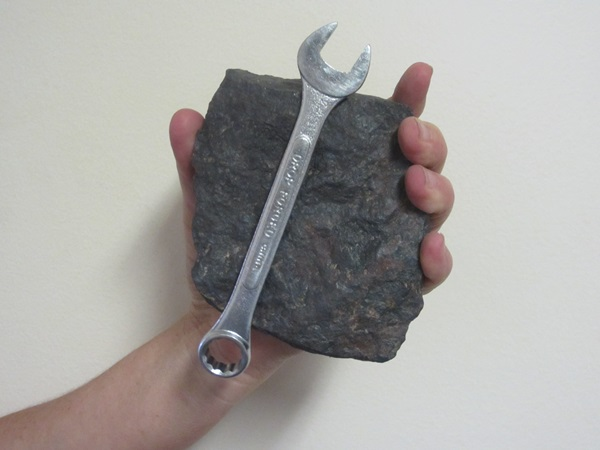
\includegraphics[width=0.98\textwidth]{./images/photos/lodestone_1.jpg}\\
    \end{center}
  \end{column}
  \begin{column}{0.52\textwidth}
        Similar properties are exhibited by
        \begin{itemize}
            \item {\bf nickel (Ni)}, \\
            \item {\bf cobalt (Co)}, \\
            \item {\bf gadolinium (Gd)}, and \\
            \item {\bf dysprosium (Dy)}. \\
        \end{itemize}
        \vspace{0.2cm}
        We call these materials {\bf ferromagnets}.
        Ferromagnetism is due to a quantum effect called
        {\em exchange coupling}.
  \end{column}
\end{columns}

\vspace{0.4cm}

Not only these materials can have a significant magnetisation when inside an external magnetic field,
they also {\bf retain their magnetisation in the absence of an external magnetic field.}

\end{frame}

%
%
%

\begin{frame}{Magnetic properties of materials}

But {\bf other substances get magnetised too.}

\begin{columns}
  \begin{column}{0.50\textwidth}
    \begin{center}
      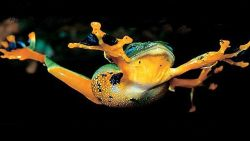
\includegraphics[width=0.90\textwidth]{./images/photos/levitating_frog_01.jpg}\\
    \end{center}
  \end{column}
  \begin{column}{0.50\textwidth}
    \begin{itemize}
      \item It might seem odd but, {\bf water} can be magnetised!
      \item {\bf Wood} can be magnetised!
      \item {\bf Frogs} can be magnetised!
      \item And, of course, {\bf you} can be magnetised too!
    \end{itemize}
  \end{column}
\end{columns}

\vspace{0.4cm}

But you can not attract wood with a horseshoe magnet.
And you need an enormous magnetic field ($\sim$ 15 T) to levitate a frog.\\

\vspace{0.3cm}

The magnetic effects for these materials are {\bf very very weak!}
\begin{itemize}
  \item $\sim$million times weaker than the effects in ferromagnetic materials.
\end{itemize}
Moreover, water, wood and frogs do not remain magnetized once the external magnetic field is removed.

\end{frame}

%
%
%

\begin{frame}{Magnetic properties of materials}

The materials that exhibit weaker and non-permanent magnetic effects
have a rather {\bf odd behaviour} in the following sense:\\

\vspace{0.3cm}

Recall that an {\bf electric field polarises a dielectric in}
(more or less) {\bf the direction of the field}.
However, in the presence of a magnetic field, some substances get
magnetised in the direction of the field and some in the opposite direction!

\vspace{0.2cm}

\begin{itemize}
  \item Substances that get {\bf magnetised in the direction of the magnetic field},
        are called {\bf \color{blue} paramagnetic}.
  \item Substances that get {\bf magnetised in the direction opposite to the magnetic field},
        are called {\bf \color{magenta} diamagnetic}.
\end{itemize}

\vspace{0.3cm}

What physics underpins that difference in the magnetic behaviour?\\

\vspace{0.2cm}

We will develop (..wrong) classical arguments to understand these effects.

\end{frame}


% starting reminder
{
\reminderslide

%
%
%

\begin{frame}{Reminder: Electric dipole moments and polarization}

\begin{columns}
  \begin{column}{0.50\textwidth}
    \begin{center}
      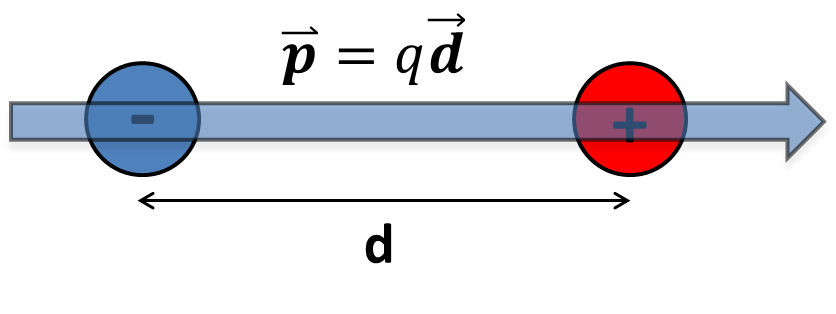
\includegraphics[width=0.98\textwidth]{./images/schematics/electric_dipole_moment_01.png}\\
    \end{center}
  \end{column}
  \begin{column}{0.50\textwidth}
   An electric dipole its described by its electric dipole moment $\vec{p}$
   (a vector, pointing from the - to the + charge):
   \begin{equation*}
     \vec{p} = q \vec{d}
   \end{equation*}
  \end{column}
\end{columns}

\begin{columns}
  \begin{column}{0.60\textwidth}
    An external electric field {\bf induces a dipole moment} in the
    direction of the field, or {\bf rotates polar molecules}
    towards the direction of the field. \\
    \vspace{0.2cm}
    The {\bf torque} $\vec{T}$ is given by: $\vec{T} = \vec{p} \times \vec{E}$
  \end{column}
  \begin{column}{0.40\textwidth}
    \begin{center}
      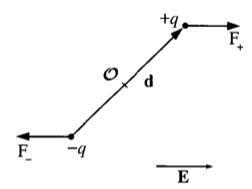
\includegraphics[width=0.70\textwidth]{./images/schematics/electric_dipole_moment_torque.png}\\
    \end{center}
  \end{column}
\end{columns}

\vspace{0.2cm}
The net effect is that matter gets {\bf polarised at a macroscopic level}
(not just at the level of individual atoms or molecules).\\
\vspace{0.2cm}
We defined the {\bf polarisation} $\vec{P}$
as the {\bf amount of electric dipole moment per unit volume}.

\end{frame}

%
%
%

\begin{frame}{Reminder: Electric dipole moments and polarization}

In a polarised material, there is accumulation of {\bf induced charge}:\\
Both {\em \bf surface} and {\em \bf volume} charge is induced.\\
\begin{columns}
  \begin{column}{0.20\textwidth}
    \begin{center}
      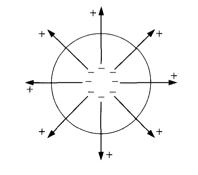
\includegraphics[width=0.92\textwidth]{./images/schematics/divergent_polarization.png}\\
    \end{center}
  \end{column}
  \begin{column}{0.80\textwidth}
    \begin{center}
       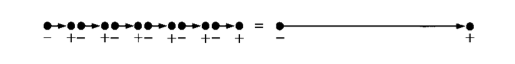
\includegraphics[width=0.95\textwidth]{./images/schematics/polarization_charges.png}\\
     \end{center}
  \end{column}
\end{columns}

We convinced ourselves that the density of the surface charge is $\displaystyle \sigma_{P} = \vec{P} \hat{n}$
where $\hat{n}$ is a unit vector normal to the surface,
whereas the density of the volume charge is $\displaystyle \rho_{P} = - \vec{\nabla} \vec{P}$.

\vspace{0.1cm}

The charges induced by polarisation,
{\bf create their own electric field $\vec{E}_{P}$ that opposes the external electric field.}
\begin{equation*}
  \vec{E}_{P}(\vec{r}) = - \vec{\nabla} V_{P}(\vec{r})
\end{equation*}
\begin{equation*}
  V_{P}(\vec{r}) =
    \frac{1}{4\pi \epsilon_0} \int \frac{1}{|\vec{r} - \pvec{r}'|} \sigma_{P} (\pvec{r}') dS^{\prime} +
    \frac{1}{4\pi \epsilon_0} \int \frac{1}{|\vec{r} - \pvec{r}'|} \rho_{P}   (\pvec{r}') d\tau^{\prime}
\end{equation*}

\end{frame}

} % ending reminder

%
%
%

\begin{frame}{Magnetic dipole moment and magnetization}

The situation in magnetism is very very similar (at least mathematically).\\
\vspace{0.2cm}

\begin{columns}
  \begin{column}{0.25\textwidth}
    \begin{center}
      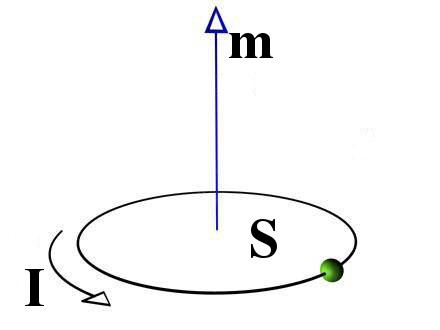
\includegraphics[width=0.95\textwidth]{./images/schematics/magnetic_dipole_moment_00.jpg}\\
    \end{center}
  \end{column}
  \begin{column}{0.70\textwidth}
    We defined the {\bf magnetic dipole moment} $\vec{m}$ as:
   \begin{equation*}
     \vec{m} = I \vec{S}
   \end{equation*}
  \end{column}
\end{columns}

\vspace{0.2cm}

An external magnetic field $\vec{B}$ exerts a torque $\vec{T}$ on a magnetic dipole $\vec{m}$ which is given by:
\begin{equation*}
  \vec{T} = \vec{m} \times \vec{B}
\end{equation*}

This will tend to {\bf align} the previously randomised {\bf magnetic moments}
and {\bf create magnetisation at a macroscopic level}.\\
\vspace{0.2cm}

We define {\bf magnetisation} $\vec{M}$ as the amount of {\bf magnetic dipole moment per unit volume}.

\end{frame}

%
%
%

\begin{frame}{Magnetization-induced currents}

The {\bf magnetisation induces surface and volume currents}.\\
\vspace{0.3cm}
We can easily be convinced, although we will not show it mathematically,
that the {\bf density of the surface current} is:
\begin{equation*}
  j_{m}^{surf} = \vec{M} \times \hat{n}
\end{equation*}

\vspace{0.1cm}

whereas the {\bf density of the volume current} is:
\begin{equation*}
  j_{m}^{vol} = \vec{\nabla} \times \vec{M}
\end{equation*}

\begin{center}
  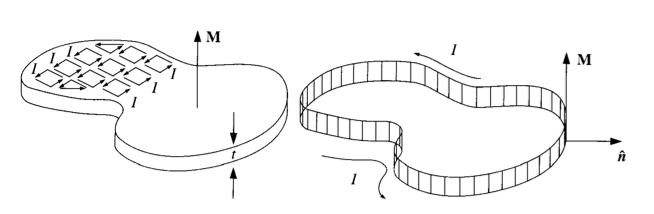
\includegraphics[width=0.98\textwidth]{./images/schematics/magnetization_currents_01.png}\\
\end{center}

\end{frame}


%
%
%

\begin{frame}{Correspondence between quantities}

{
\setlength{\extrarowheight}{14pt}
\setlength{\arraycolsep}{5pt}

\begin{center}
  \begin{table}[H]
    \begin{tabular}{c|c||c|c}
      \hline
      \multicolumn{2}{c||}{\bf Electrostatics} &
      \multicolumn{2}{c}  {\bf Magnetostatics} \\
      \hline
         {\scriptsize electric dipole moment} &
         $\vec{p} = q \vec{d}$ &
         $\vec{m} = I \vec{S}$ &
         {\scriptsize magnetic dipole moment} \\
      \hline
         {\scriptsize torque within $\vec{E}$ field} &
         $\vec{T} = \vec{p} \times \vec{E}$ &
         $\vec{T} = \vec{m} \times \vec{B}$ &
         {\scriptsize torque within a $\vec{B}$ field} \\
      \hline
         {\scriptsize polarization} &
         $\vec{P}  = \frac{(e.d.m)}{volume}$ &
         $\vec{M} = \frac{(m.d.m)}{volume}$ &
         {\scriptsize magnetization} \\
      \hline
         {\scriptsize surface charge density} &
         $\sigma_{P} = \vec{P} \hat{n}$ &
         $j_{m}^{surf} = \vec{M} \times \hat{n}$ &
         {\scriptsize surface current density} \\
      \hline
         {\scriptsize volume charge density} &
         $\rho_{P} = - \vec{\nabla} \vec{P}$ &
         $j_{m}^{vol} = \vec{\nabla} \times \vec{M}$ &
         {\scriptsize volume current density} \\
      \hline
    \end{tabular}
  \end{table}
\end{center}
}

\end{frame}

%
%
%

\begin{frame}{Ampere's law in materials}

Recall {\bf Ampere's law in vacuum}:
\begin{equation*}
  \oint_{L} \vec{B} d\vec{\ell} = \mu_0 \int_{S(L)} \vec{j} d\vec{S} \;\;
  {\color{blue}(integral\;form)},
  \;\;\;\;\;
  \vec{\nabla} \times \vec{B} = \mu_0 \vec{j} \;\;
  {\color{blue}(differential\;form)}
\end{equation*}

Ampere's law,
\begin{itemize}
     \item in integral form, connects the line integral of the
               magnetic field $\vec{B}$ along a closed path L with the current I
               flowing through the surface S(L) defined by the closed path L, and,
     \item in differential form, connects the rotation of the magnetic field,
               at any point in space, with the local current density $\vec{j}$.\\
 \end{itemize}

\vspace{0.2cm}

Our {\bf objective is to re-formulate Ampere's law for materials} where, \\
{\bf in addition to free currents}, we have {\bf magnetization-induced currents}.\\

\vspace{0.2cm}
Recall that we did something very similar with Gauss's law in electrostatics. \\

\end{frame}


% starting reminder
{
\reminderslide

%
%
%

\begin{frame}{Reminder: Gauss' law in materials}

We started from Gauss’ law in vacuum:
\begin{equation*}
  \vec{\nabla} \vec{E} = \frac{\rho}{\epsilon_0}
\end{equation*}

and wrote the total charge density $\rho$ as the sum of the free ($\rho_{f}$)
and polarisation ($\rho_{P}$) charge densities:
\begin{equation*}
  \vec{\nabla} \vec{E} = \frac{\rho_{f} + \rho_{P}}{\epsilon_0}
\end{equation*}

The polarisation charge density $\rho_{P}$ is given, in terms of the polarisation field $\vec{P}$, by:
\begin{equation*}
  \rho_{P} = - \vec{\nabla}\vec{P}
\end{equation*}

and, therefore, Gauss' law becomes:
\begin{equation*}
  \vec{\nabla} \vec{E} = \frac{\rho_{f} - \vec{\nabla}\vec{P}}{\epsilon_0}
\end{equation*}

\end{frame}

%
%
%

\begin{frame}{Reminder: Gauss' law in materials}

We collected all the divergences together and we obtained:
\begin{equation*}
  \vec{\nabla} \Big( \epsilon_0 \vec{E} + \vec{P} \Big) = \rho_{f}
\end{equation*}

This is the differential form of Gauss's law in materials.\\
\vspace{0.2cm}

We defined the electric displacement $\vec{D}$ as:
\begin{equation*}
  \vec{D} = \epsilon_0 \vec{E} + \vec{P}
\end{equation*}

and, therefore, Gauss's law in materials was written as:
\begin{equation*}
  \vec{\nabla} \vec{D} = \rho_{f}
\end{equation*}

In integral form,  Gauss's law in materials becomes:
\begin{equation*}
  \oint_{S} \vec{D} d\vec{S} = \int_{\tau(S)} \rho_{f} d\tau = Q_{f}
\end{equation*}

\end{frame}

} % ending reminder

%
%
%
%

\begin{frame}{Ampere's law in materials}

Similarly, starting from Ampere's law in vacuum:
\begin{equation*}
  \vec{\nabla} \times \vec{B} = \mu_0 \vec{j}
\end{equation*}

we can write the total current density $\vec{j}$ as the vector sum of the free ($\vec{j}_{f}$)
and magnetization ($\vec{j}_{m}$) current densities:
\begin{equation*}
  \vec{\nabla} \times \vec{B} = \mu_0 \Big( \vec{j}_{f} + \vec{j}_{m} \Big)
\end{equation*}

Expressing the magnetization current density $\vec{j}_{m}$ in terms of the
magnetization field $\vec{M}$:
\begin{equation*}
  \vec{j}_{m} = \vec{\nabla} \times \vec{M}
\end{equation*}

we can write Ampere's law as:
\begin{equation*}
  \vec{\nabla} \times \vec{B} = \mu_0 \Big( \vec{j}_{f} + \vec{\nabla} \times \vec{M} \Big)
\end{equation*}

\end{frame}


%
%
%

\begin{frame}{Ampere's law in materials}

Dividing with $\mu_0$ and collecting the curls together and get:
\begin{equation*}
  \vec{\nabla} \times \frac{\vec{B}}{\mu_0} = \vec{j}_{f} + \vec{\nabla} \times \vec{M} \Rightarrow
  \vec{\nabla} \times \Big( \frac{\vec{B}}{\mu_0} - \vec{M} \Big) = \vec{j}_{f}
\end{equation*}

We define the {\bf magnetic field strength} or {\bf magnetic field intensity} $\vec{H}$ as:
\begin{equation*}
  \vec{H} = \frac{\vec{B}}{\mu_0} - \vec{M}
\end{equation*}

we can write the differential form of Ampere's law in materials as:
\begin{equation*}
  \vec{\nabla} \times \vec{H} = \vec{j}_{f}
\end{equation*}

Using Stokes' theorem, as we have done several times in past lectures,
we can go to the integral form of Ampere's law in materials which is:
\begin{equation*}
  \oint_{L} \vec{H} d\vec{\ell} = \int_{S(L)} \vec{j}_{f} d\vec{S} = I_{f}
\end{equation*}

\end{frame}

%
%
%

\begin{frame}{The ``{\em H field}''}

In SI, the quantity $\displaystyle \vec{H} = \frac{\vec{B}}{\mu_0} - \vec{M}$ has {\bf units of A/m}.\\
\vspace{0.1cm}

$\vec{H}$ plays a role analogous to $\vec{D}$ in electrostatics:
It allows us to write Ampere's law in terms of the free currents alone.\\
\vspace{0.1cm}

We called $\vec{H}$ {\bf magnetic field strength} or {\bf magnetic field intensity}.\\
\begin{itemize}
{\small
\item
Some textbooks also call $\vec{H}$ the ... {\bf auxiliary field}.\\
\item
Other textbooks call $\vec{H}$ the {\bf magnetic field}, and then call $\vec{B}$ something else
(typically, magnetic induction). Confusion is inevitabe!\\
\item
Sometimes, $\vec{H}$ is called the {\bf magnetising field} - I like this best.\\
\item
Griffiths makes a good suggestion:
{\em "H has no sensible name. Just call it H."} (at least we all agree on the symbol).\\
}
\end{itemize}

\vspace{0.1cm}

Typically, it is easier to think in terms of  $\vec{H}$ and $\vec{E}$:
At the Lab we control free currents (hence $\vec{H}$) and the voltage of EMF sources (hence $\vec{E}$).\\
But let's not be confused: {\bf $\vec{B}$ and $\vec{E}$ are the fundamental quantities}.

\end{frame}


% starting reminder
{
\reminderslide

%
%
%

\begin{frame}{Reminder: Electric susceptibility}

The Gauss' law in materials is:
$\displaystyle \vec{\nabla} \Big( \epsilon_0 \vec{E} + \vec{P} \Big) = \rho_{f}$\\

\vspace{0.2cm}

The polarisation vector $\vec{P}$ can be expressed in terms of $\vec{E}$:
\begin{equation*}
  \vec{P} = \chi_e \epsilon_0 \vec{E}
\end{equation*}
where $\chi_e$ is the so-called {\bf electric susceptibility} (dimensionless).\\

\vspace{0.2cm}

For {\bf linear dielectrics} (and low intensity fields) $\chi_e$ is a
constant that does not depend on $\vec{E}$.
Therefore, Gauss' law can be written as:
\begin{equation*}
  \vec{\nabla} \Big( \epsilon_0 \vec{E} + \chi_e \epsilon_0 \vec{E} \Big) = \rho_{f} \Rightarrow
  (1+\chi_e) \epsilon_0 \vec{\nabla} \vec{E} = \rho_{f} \Rightarrow
  \epsilon_r \epsilon_0 \vec{\nabla} \vec{E} = \rho_{f} \Rightarrow
  {\color{magenta}
     \epsilon \vec{\nabla} \vec{E} =  \rho_{f}
  }
\end{equation*}
where the factor $\epsilon_r = 1+\chi_e$
is the {\bf relative permittivity} or {\bf dielectric constant} (dimensionless) and
$\epsilon = \epsilon_r  \epsilon_0$ is the {\bf permittivity} of the dielectric
(SI unit: $A \cdot s \cdot  V^{-1} \cdot m^{-1}$).\\

\end{frame}

} % ending reminder

%
%
%

\begin{frame}{Magnetic susceptibility}

Ampere's law in materials is:
$\displaystyle \vec{\nabla} \times \Big( \frac{\vec{B}}{\mu_0} - \vec{M} \Big) = \mu_0 \vec{j}_{f}$\\
\vspace{0.1cm}

If the analogy with electrostatics was exact,
we would write $\vec{M}$ in terms of $\vec{B}$.
However, this is where the analogy breaks.
Instead we typically write:
\begin{equation*}
{\color{magenta}
  \vec{M} = \chi_{m} \vec{H}
}
\end{equation*}
where  $\chi_m$ is the {\bf magnetic susceptibility}.
For {\bf linear materials}, $\chi_m$ is a constant independent of the value of $\vec{H}$.
Expressing $\vec{B}$ in terms of $\vec{H}$:
\begin{equation*}
  \vec{H} = \frac{\vec{B}}{\mu_0} - \vec{M} \Rightarrow
  \vec{B} = \mu_0 \Big( \vec{H} + \vec{M} \Big) \xRightarrow{\vec{M} = \chi_{m} \vec{H}}
  \vec{B} = \Big(1 + \chi_{m} \Big) \mu_0  \vec{H} \Rightarrow
\end{equation*}
\begin{equation*}
  \vec{B} = \mu_r \mu_0 \vec{H} \Rightarrow
  {\color{magenta}
    \vec{B} = \mu \vec{H}
  }
\end{equation*}
where $\mu_r = 1+\chi_{\mu}$
is the {\bf relative permeability} (dimensionless) and
$\mu = \mu_r  \mu_0$ is the {\bf permeability} of the material
(SI unit: $V \cdot s \cdot  A^{-1} \cdot m^{-1}$).\\

\end{frame}


%
%
%

\begin{frame}{Correspondence between quantities}

{
\setlength{\extrarowheight}{8pt}
\setlength{\arraycolsep}{5pt}

\begin{center}
  \begin{table}[H]
    \begin{tabular}{c|c||c|c}
      \hline
      \multicolumn{2}{c||}{\bf Electrostatics} &
      \multicolumn{2}{c}  {\bf Magnetostatics} \\
      \hline
         {\scriptsize electric dipole moment} &
         $\vec{p} = q \vec{d}$ &
         $\vec{m} = I \vec{S}$ &
         {\scriptsize magnetic dipole moment} \\
      \hline
         {\scriptsize torque within $\vec{E}$ field} &
         $\vec{T} = \vec{p} \times \vec{E}$ &
         $\vec{T} = \vec{m} \times \vec{B}$ &
         {\scriptsize torque within a $\vec{B}$ field} \\
      \hline
         {\scriptsize polarization} &
         $\vec{P}  = \frac{(e.d.m)}{volume}$ &
         $\vec{M} = \frac{(m.d.m)}{volume}$ &
         {\scriptsize magnetization} \\
      \hline
         {\scriptsize surface charge density} &
         $\sigma_{P} = \vec{P} \hat{n}$ &
         $j_{m}^{surf} = \vec{M} \times \hat{n}$ &
         {\scriptsize surface current density} \\
      \hline
         {\scriptsize volume charge density} &
         $\rho_{P} = - \vec{\nabla} \vec{P}$ &
         $j_{m}^{vol} = \vec{\nabla} \times \vec{M}$ &
         {\scriptsize volume current density} \\
      \hline
         {\scriptsize electric displacement} &
         $\vec{D} = \epsilon_0 \vec{E} + \vec{P}$ &
         $\vec{H} = \frac{\vec{B}}{\mu_0} - \vec{M}$ &
         {\scriptsize magnetizing field} \\
      \hline
         \multirow{2}{*}{\scriptsize Gauss' law in materials} &
         $\vec{\nabla} \vec{D} = \rho_{f}$ &
         $\vec{\nabla} \times \vec{H} = \vec{j}_{f}$ &
         \multirow{2}{*}{\scriptsize Ampere's law in materials} \\
      \hhline{~--~}
         &
         $\oint_{S} \vec{D} d\vec{S} = Q_{f}$ &
         $\oint_{L} \vec{H} d\vec{\ell} = I_{f}$ &
         \\
      \hline
    \end{tabular}
  \end{table}
\end{center}
}

\end{frame}

%
%
%

\begin{frame}{Maxwell's equations we know so far}

{\small

\begin{center}
{
  \begin{table}[H]
    \begin{tabular}{|l|c|c|}
      \hline
        \multicolumn{3}{|l|} {
          {\color{magenta}
           {\bf Static case in vacuum}
          }
        }\\
      \hline
      {\bf Gauss's law} &
        $\displaystyle \oint \vec{E} d\vec{S} = \frac{1}{\epsilon_0} \int \rho d\tau = \frac{Q}{\epsilon_0}$ &
        $\displaystyle \vec{\nabla} \cdot \vec{E} = \frac{\rho}{\epsilon_0}$ \\

      {\bf Circuital law} &
        $\displaystyle \oint \vec{E} d\vec{\ell} = 0$ &
        $\displaystyle \vec{\nabla} \times \vec{E} = 0$ \\

      no mag. monopoles &
        $\displaystyle \oint \vec{B} d\vec{S} = 0$ &
        $\displaystyle \vec{\nabla} \cdot \vec{B} = 0$ \\

      {\bf Ampere's law} &
        $\displaystyle \oint \vec{B} d\vec{\ell} = \mu_{0} \int \vec{j} d\vec{S} = \mu_0 I$ &
        $\displaystyle \vec{\nabla} \times \vec{B} = \mu_{0} \vec{j}$ \\

      \hline
    \end{tabular}
  \end{table}
}
\end{center}

\begin{center}
{
  \begin{table}[H]
    \begin{tabular}{|l|c|c|}
      \hline
        \multicolumn{3}{|l|} {
          {\color{magenta}
           {\bf Static case within materials}
          }
        }\\
      \hline
      {\bf Gauss's law} &
        $\displaystyle \oint \vec{D} d\vec{S} =  \int \rho_{f} d\tau = Q_{f}$ &
        $\displaystyle \vec{\nabla} \cdot \vec{D} = \rho_{f}$ \\

      {\bf Circuital law} &
        $\displaystyle \oint \vec{E} d\vec{\ell} = 0$ &
        $\displaystyle \vec{\nabla} \times \vec{E} = 0$ \\

      no mag. monopoles &
        $\displaystyle \oint \vec{B} d\vec{S} = 0$ &
        $\displaystyle \vec{\nabla} \cdot \vec{B} = 0$ \\

      {\bf Ampere's law} &
        $\displaystyle \oint \vec{H} d\vec{\ell} =  \int \vec{j}_{f} d\vec{S} = I_{f}$ &
        $\displaystyle \vec{\nabla} \times \vec{H} = \vec{j}_{f}$ \\
      \hline
    \end{tabular}
  \end{table}
}
\end{center}

}

\end{frame}

%
%
%

\begin{frame}{Diamagnetic materials}

In {\bf diamagnetic} substances, the magnetization is in a direction
{\bf opposite} to that of an externally applied magnetizing field.
\begin{itemize}
  \item Diamagnetism is a {\bf weak and non-permanent effect}.
  \item Diamagnetic materials are {\bf repelled} by the applied magnetic field.
\end{itemize}
\vspace{0.3cm}

\begin{columns}
  \begin{column}{0.25\textwidth}
   \begin{block}{}
     Reminder:
     \begin{equation*}
       \vec{M} = \chi_{m} \vec{H}
     \end{equation*}
     \begin{equation*}
       \vec{B} = \mu \vec{H}
     \end{equation*}
     \begin{equation*}
        \mu = \mu_0 \Big(1 + \chi_{m} \Big)
     \end{equation*}
   \end{block}
  \end{column}
  \begin{column}{0.05\textwidth}
  \end{column}
  \begin{column}{0.70\textwidth}
     Since $\vec{M}$ and $\vec{H}$ are anti-parallel: $\chi_{m} < 0$\\
     \vspace{0.2cm}
     Diamagnetism is a weak effect: $|\chi_{m}| << 1$\\
     and, therefore: $\mu / \mu_{0} < 1$\\
     \vspace{0.2cm}
     Typical values of $\chi_m$ for diamagnetic substances:
     \begin{center}
       \begin{table}[H]
         \begin{tabular}{|l|l|}
         \hline
           Substance &  $\chi_m$ at $T=0^{o}C$ \\
         \hline
           $H_{2}$  & $-2.3 \cdot 10^{-9}$ \\
           $H_{2}O$ & $-1.2 \cdot 10^{-5}$ \\
           $N_{2}$  & $-0.7 \cdot 10^{-8}$ \\
           $Ag$     & $-2.5 \cdot 10^{-5}$ \\
         \hline
         \end{tabular}
       \end{table}
     \end{center}
  \end{column}
\end{columns}

\end{frame}

%
%
%

\begin{frame}{Paramagnetic materials}

In {\bf paramagnetic} substances, the magnetization is in the same direction
as that of an externally applied magnetizing field.
\begin{itemize}
  \item Paramagnetism is a {\bf weak and non-permanent effect}.\\
  \item Paramagnetic materials are {\bf attracted} by the applied magnetic field.
\end{itemize}
\vspace{0.3cm}

\begin{columns}
  \begin{column}{0.25\textwidth}
   \begin{block}{}
     Reminder:
     \begin{equation*}
       \vec{M} = \chi_{m} \vec{H}
     \end{equation*}
     \begin{equation*}
       \vec{B} = \mu \vec{H}
     \end{equation*}
     \begin{equation*}
        \mu = \mu_0 \Big(1 + \chi_{m} \Big)
     \end{equation*}
   \end{block}
  \end{column}
  \begin{column}{0.05\textwidth}
  \end{column}
  \begin{column}{0.70\textwidth}
     Since $\vec{M}$ and $\vec{H}$ are parallel: $\chi_{m} > 0$\\
     \vspace{0.2cm}
     Paramagnetism is a weak effect: $|\chi_{m}| << 1$\\
     and, therefore: $\mu / \mu_{0} > 1$\\
     \vspace{0.2cm}
     Typical values of $\chi_m$ for paramagnetic substances:
     \begin{center}
       \begin{table}[H]
         \begin{tabular}{|l|l|}
         \hline
           Substance &  $\chi_m$ at $T=20^{o}C$ \\
         \hline
           $O_{2}$  & $1.8 \cdot 10^{-8}$ \\
           $Pt$     & $2.7 \cdot 10^{-5}$ \\
           $Al$     & $2.1 \cdot 10^{-5}$ \\
         \hline
         \end{tabular}
       \end{table}
     \end{center}
  \end{column}
\end{columns}

\end{frame}

%
%
%

\begin{frame}{Ferromagnetic materials}

For {\bf ferromagnetic} materials, the {\bf magnetisation} produced by an external field is {\bf much much larger}.

\begin{itemize}
{\small
  \item Previously quoted values of the magnetic susceptibility
           for paramagnetic and diamagnetic materials that were at most in the few $\times$ $10^{-5}$ range.
  \item For iron, nickel and Cobalt, the magnetic susceptibility is $\sim 10^{+6}$!
}
\end{itemize}

\vspace{0.2cm}

In ferromagnetic materials the {\bf magnetic susceptibility is not a constant}
\begin{itemize}
   \item i.e. ferromagnets are not linear materials.
\end{itemize}

As matter of fact,  the {\bf magnetic susceptibility does not have a single value for a given M and H!}
\begin{itemize}
   \item i.e. the magnetisation depends on its magnetisation history!
\end{itemize}

\vspace{0.2cm}

Ferromagnetic materials {\bf retain a magnetisation} even when the magnetising field is removed!

\end{frame}

%
%
%

\begin{frame}{Hysteresis loop}

\begin{columns}
  \begin{column}{0.30\textwidth}
    \begin{center}
       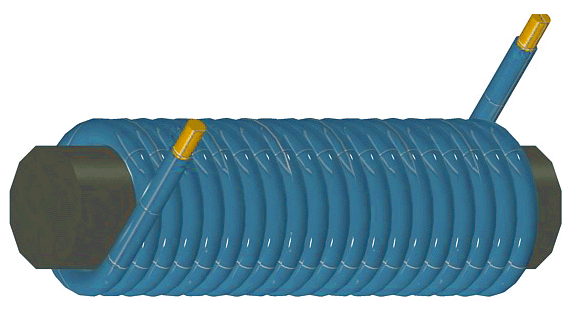
\includegraphics[width=0.85\textwidth]{./images/schematics/simple_electromagnet_01.png}\\
    \end{center}
  \end{column}
  \begin{column}{0.70\textwidth}
   {\small
       Consider the simple electromagnet shown on the left. Current I running in the coil turns
       creates a magnetic field and magnetizes an iron core.
       Let's consider the magnetization M as function of the current intensity I.
   }
  \end{column}
\end{columns}

\begin{center}
   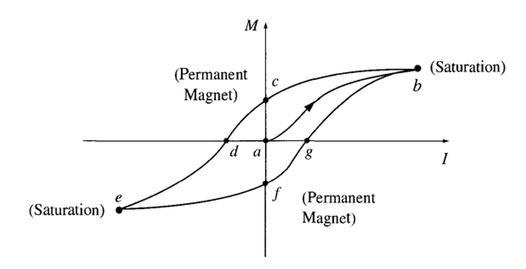
\includegraphics[width=0.98\textwidth]{./images/schematics/hysterisis_curve_01.png}\\
\end{center}

\end{frame}

%
% Physical origins
%

\begin{frame}{Physical origins}

What physics underpins the different magnetic behaviour
of diamagnetic, paramagnetic and ferromagnetic materials?\\
\vspace{0.2cm}

I will attempt to give some {\bf classical arguments} and descriptions aiming to develop a
qualitative understanding.\\
\vspace{0.2cm}

But, keep in mind that, our classical explanations, although simple and intuitive,
are {\bf ultimately wrong}.

\begin{itemize}
  \item
    They are {\bf quantum-mechanical effects}.
    A detailed description of diamagnetism, paramagnetism and ferromagnetism
    is beyond the scope of this introductory course.
  \item
    In fact, our explanation is wrong even in the context of classical physics
    (See {\it `Classical physics gives neither diamagnetism nor paramagnetism', Section 34.6 in Feynman lectures, available online}).
\end{itemize}

But we will stick to these classical arguments for now.

\end{frame}

%
%
%

\begin{frame}{Physical origin of diamagnetism}

Consider an electron orbiting a nucleus anticlockwisely on the xy plane:\\
A {\bf magnetic dipole moment} is associated with the orbital motion:
\begin{equation*}
  \vec{m} = - \frac{1}{2} e u R \hat{z}
\end{equation*}

If a magnetic field $\vec{B}$ is applied, the magnetic moment changes
in a direction {\bf opposite to the magnetic field} (See `Optional reading'):
\begin{equation*}
    {\Delta}\vec{m} =
      - \frac{e^2 R^2}{4m_e} \vec{B}
\end{equation*}

Electrons rotate around the nucleus in {\bf random directions}:
There is no net magnetization as their {\bf magnetic dipole moments cancel out}.\\
\vspace{0.1cm}

In an external field,
${\Delta}\vec{m}$ is {\bf antiparallel to that field for \underline{all} electrons}:
This creates {\bf net magnetisation opposite to the external field}.\\
\vspace{0.1cm}

Diamagnetism is a {\bf universal phenomenon}.
\begin{itemize}
  \item It occurs in all substances, even paramagnetic ones.
%  \item But for paramagnetic substances there is also a stronger and opposite phenomenon at work.
\end{itemize}

\end{frame}

%
%
%

\begin{frame}{Physical origin of paramagnetism}

Just as the orbital angular momentum of the electron
is responsible for a magnetic dipole moment, {\bf so is its spin}!
\begin{itemize}
{\small
  \item Nothing "spins". Spin is an {\em intrinsic} angular momentum of the electron.
  \item So, intrinsically, {\em every electron is a small magnetic dipole}.
}
\end{itemize}

\vspace{0.1cm}

In the atomic shells, electrons are arranged {\bf in pairs of opposite spin}:
The intrinsic magnetic dipole moments of the pair are canceled out.\\
\vspace{0.2cm}

But in atoms with {\bf odd number} of electrons, there is an {\bf unmatched electron}:
Its intrinsic magnetic dipole moment is not canceled out.\\
\vspace{0.2cm}

In the presence of a magnetic field, {\bf the unmatched electron in each atom}, feels a
torque ($T = \vec{m} \times \vec{B}$) and it is {\bf aligned with field}:
This creates a  net macroscopic {\bf magnetisation along the field}.\\
\vspace{0.2cm}

Realigning the spin of an electron is easier than rearranging the atomic orbits.
Thus, even though diamagnetism is universal, paramagnetism is the dominant effect for some substances.

\end{frame}

%
%
%

\begin{frame}{Physical origin of ferromagnetism}

{\bf Ferromagnetism}, like paramagnetism, involves
 the magnetic dipole moments due to the {\bf spin of unpaired atomic electrons}.\\

\vspace{0.1cm}

\begin{columns}
  \begin{column}{0.55\textwidth}
    \begin{center}
       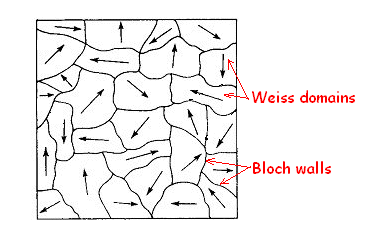
\includegraphics[width=0.85\textwidth]{./images/schematics/weiss_domains_01.png}\\
    \end{center}
  \end{column}
  \begin{column}{0.45\textwidth}
       Within regions (called {\em Weiss} domains),
       every magnetic dipole {\em prefers} to be aligned at the same direction as its neighbours.
       Therefore, each Weiss domain has a macroscopic magnetisation.\\
  \end{column}
\end{columns}

\vspace{0.1cm}

For a sizeable chunk of material,
there is a large numbers of domains magnetized at random directions (*)
so there is {\bf no net magnetisation}.\\

\vspace{0.1cm}

\noindent\rule{2cm}{0.4pt}\\
{\scriptsize
 (*) actually, there may be preferential direction within a crystal,
     but a sizeable chunk of material contains a large number or randomly oriented crystals.\\
}

\end{frame}


%
%
%

\begin{frame}{Physical origin of ferromagnetism}

A magnetic field $\vec{B}$ will try to align each dipole with it
($\vec{T} = \vec{m} \times \vec{B}$), but dipoles prefer to stay aligned with their neighbours.\\

\vspace{0.1cm}

Now, consider dipoles neighbouring Weiss domains whose magnetization is already in the direction of $\vec{B}$.
These dipole would feel:
\begin{itemize}
\item the influence of the torque due to $\vec{B}$, and
\item the influence of the neighbouring dipoles already aligned with $\vec{B}$.
\end{itemize}
The end result is that {\bf  Weiss domains re-arrange their boundaries}.\\
Domains with magnetization in the direction of $\vec{B}$ grow - others shrink.\\
There is now {\bf net magnetisation towards $\vec{B}$}.\\

\begin{center}
   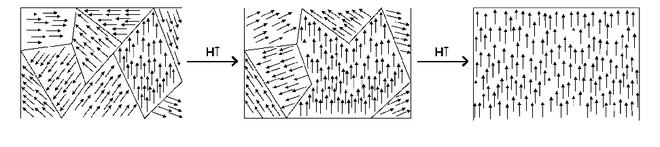
\includegraphics[width=0.96\textwidth]{./images/schematics/weiss_domains_02.png}\\
\end{center}

\end{frame}

%
%
%

\begin{frame}{Physical origin of ferromagnetism}

Random thermal motions tend to destroy the ordering / dipole alignment.
\begin{itemize}
   \item Random thermal motion increases with temperature.
\end{itemize}

\vspace{0.2cm}

There is a given temperature called {\bf Curie point} (for iron this is at 770$^{o}$ C)
where a ferromagnetic material undergoes a {\bf phase transition} and
becomes paramagnetic.\\

\begin{center}
   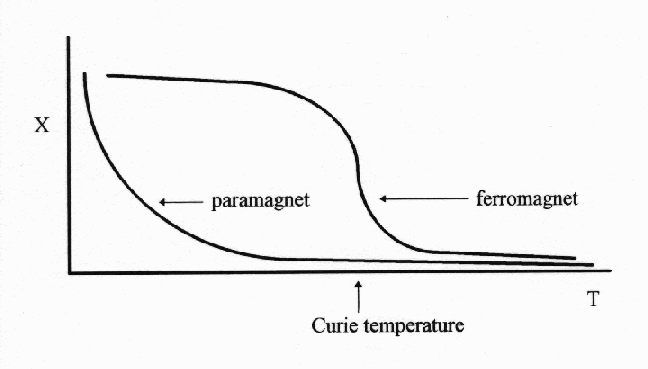
\includegraphics[width=0.75\textwidth]{./images/schematics/curie_temperature_01.png}\\
\end{center}

\end{frame}



% ------------------------------------------------------------------------------
% ------------------------------------------------------------------------------

%
% What to remember
%

\renewcommand{\lecturesummarytitle}{Main points to remember }

\renewcommand{\summarizedlecture}{7 }

%
%
%

\begin{frame}{Lecture \summarizedlecture revision}

In the last lecture:\\

\begin{itemize}

   \item We completed the study of {\bf Maxwell's eqs. in materials (for static fields)}
             and emphasized the analogies between electrostatics and magnetostatics.

   \vspace{0.2cm}

   \item We discussed the magnetic properties of materials
             ({\bf diamagnetism}, {\bf paramagnetism} and {\bf ferromagnetism})
             and developed arguments to understand the physical origins.

   \vspace{0.2cm}

   \item We found out how to {\bf extend Maxwell's eqs. in vacuum}
             in the case of {\bf time-dependent fields}.

\end{itemize}

\end{frame}

%
%
%

\begin{frame}{Lecture \summarizedlecture revision (Magnetic moment / magnetization)}

\begin{columns}
  \begin{column}{0.25\textwidth}
    \begin{center}
      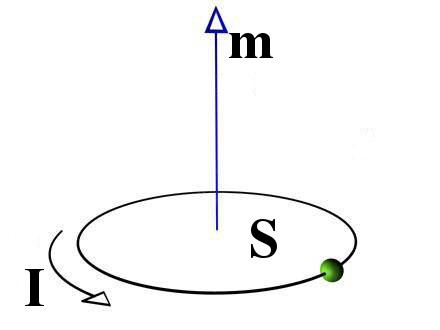
\includegraphics[width=0.95\textwidth]{./images/schematics/magnetic_dipole_moment_00.jpg}\\
    \end{center}
  \end{column}
  \begin{column}{0.70\textwidth}
    We defined the {\bf magnetic dipole moment} $\vec{m}$ as:
   \begin{equation*}
     \vec{m} = I \vec{S}
   \end{equation*}
  \end{column}
\end{columns}

\vspace{0.2cm}

An external magnetic field $\vec{B}$ exerts a torque $\vec{T}$ on a magnetic dipole $\vec{m}$ which is given by:
\begin{equation*}
  \vec{T} = \vec{m} \times \vec{B}
\end{equation*}

This will tend to {\bf align} the previously randomised {\bf magnetic moments}
and {\bf create magnetisation at a macroscopic level}.\\
\vspace{0.2cm}

We define {\bf magnetisation} $\vec{M}$ as the amount of {\bf magnetic dipole moment per unit volume}.

\end{frame}

%
%
%

\begin{frame}{Lecture \summarizedlecture revision (Magnetization-induced currents)}

The {\bf magnetisation induces surface and volume currents}.\\
\vspace{0.3cm}
We can easily be convinced, although we will not show it mathematically,
that the {\bf density of the surface current} is:
\begin{equation*}
  j_{m}^{surf} = \vec{M} \times \hat{n}
\end{equation*}

\vspace{0.1cm}

whereas the {\bf density of the volume current} is:
\begin{equation*}
  j_{m}^{vol} = \vec{\nabla} \times \vec{M}
\end{equation*}

\begin{center}
  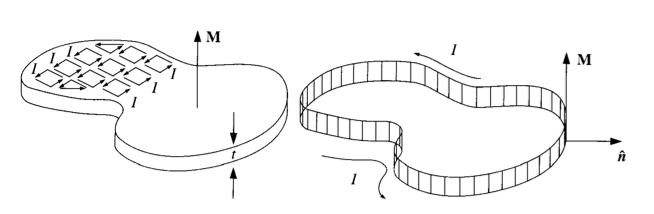
\includegraphics[width=0.98\textwidth]{./images/schematics/magnetization_currents_01.png}\\
\end{center}

\end{frame}

%
%
%

\begin{frame}{Lecture \summarizedlecture revision (Ampere's law in materials)}

We started from Ampere's law in vacuum:
\begin{equation*}
  \vec{\nabla} \times \vec{B} = \mu_0 \vec{j}
\end{equation*}
By writing the total current density $\vec{j}$ as the vector sum of the free ($\vec{j}_{f}$)
and magnetization ($\vec{j}_{m}$) current densities,
and expressing $\vec{j}_{m}$ in terms of the
magnetization field $\vec{M}$ ($\displaystyle \vec{j}_{m} = \vec{\nabla} \times \vec{M}$),
we finally wrote Ampere's law as:
\begin{equation*}
  \vec{\nabla} \times \Big( \frac{\vec{B}}{\mu_0} - \vec{M} \Big) = \vec{j}_{f}
\end{equation*}

We defined the {\bf magnetic field strength} or {\bf magnetic field intensity} $\vec{H}$ as:
\begin{equation*}
  \vec{H} = \frac{\vec{B}}{\mu_0} - \vec{M}
\end{equation*}
In SI, the quantity $\displaystyle \vec{H} = \frac{\vec{B}}{\mu_0} - \vec{M}$ has {\bf units of A/m}.\\

\end{frame}

%
%
%

\begin{frame}{Lecture \summarizedlecture revision (Linear materials)}

Ampere's law in materials is:
$\displaystyle \vec{\nabla} \times \Big( \frac{\vec{B}}{\mu_0} - \vec{M} \Big) = \mu_0 \vec{j}_{f}$\\
\vspace{0.1cm}

If the analogy with electrostatics was exact,
we would write $\vec{M}$ in terms of $\vec{B}$.
However, this is where the analogy breaks.
Instead we typically write:
\begin{equation*}
{\color{magenta}
  \vec{M} = \chi_{m} \vec{H}
}
\end{equation*}
where  $\chi_m$ is the {\bf magnetic susceptibility}.
For {\bf linear materials}, $\chi_m$ is a constant independent of the value of $\vec{H}$.
Expressing $\vec{B}$ in terms of $\vec{H}$:
\begin{equation*}
  \vec{H} = \frac{\vec{B}}{\mu_0} - \vec{M} \Rightarrow
  \vec{B} = \mu_0 \Big( \vec{H} + \vec{M} \Big) \xRightarrow{\vec{M} = \chi_{m} \vec{H}}
  \vec{B} = \Big(1 + \chi_{m} \Big) \mu_0  \vec{H} \Rightarrow
\end{equation*}
\begin{equation*}
  \vec{B} = \mu_r \mu_0 \vec{H} \Rightarrow
  {\color{magenta}
    \vec{B} = \mu \vec{H}
  }
\end{equation*}
where $\mu_r = 1+\chi_{\mu}$
is the {\bf relative permeability} (dimensionless) and
$\mu = \mu_r  \mu_0$ is the {\bf permeability} of the material
(SI unit: $V \cdot s \cdot  A^{-1} \cdot m^{-1}$).\\

\end{frame}

%
%
%

\begin{frame}{Lecture \summarizedlecture revision (Correspondence between quantities)}

{
\setlength{\extrarowheight}{8pt}
\setlength{\arraycolsep}{5pt}

\begin{center}
  \begin{table}[H]
    \begin{tabular}{c|c||c|c}
      \hline
      \multicolumn{2}{c||}{\bf Electrostatics} &
      \multicolumn{2}{c}  {\bf Magnetostatics} \\
      \hline
         {\scriptsize electric dipole moment} &
         $\vec{p} = q \vec{d}$ &
         $\vec{m} = I \vec{S}$ &
         {\scriptsize magnetic dipole moment} \\
      \hline
         {\scriptsize torque within $\vec{E}$ field} &
         $\vec{T} = \vec{p} \times \vec{E}$ &
         $\vec{T} = \vec{m} \times \vec{B}$ &
         {\scriptsize torque within a $\vec{B}$ field} \\
      \hline
         {\scriptsize polarization} &
         $\vec{P}  = \frac{(e.d.m)}{volume}$ &
         $\vec{M} = \frac{(m.d.m)}{volume}$ &
         {\scriptsize magnetization} \\
      \hline
         {\scriptsize surface charge density} &
         $\sigma_{P} = \vec{P} \cdot \hat{n}$ &
         $j_{m}^{surf} = \vec{M} \times \hat{n}$ &
         {\scriptsize surface current density} \\
      \hline
         {\scriptsize volume charge density} &
         $\rho_{P} = - \vec{\nabla} \cdot \vec{P}$ &
         $j_{m}^{vol} = \vec{\nabla} \times \vec{M}$ &
         {\scriptsize volume current density} \\
      \hline
         {\scriptsize electric displacement} &
         $\vec{D} = \epsilon_0 \vec{E} + \vec{P}$ &
         $\vec{H} = \frac{\vec{B}}{\mu_0} - \vec{M}$ &
         {\scriptsize magnetizing field} \\
      \hline
         \multirow{2}{*}{\scriptsize Gauss' law in materials} &
         $\vec{\nabla} \cdot \vec{D} = \rho_{f}$ &
         $\vec{\nabla} \times \vec{H} = \vec{j}_{f}$ &
         \multirow{2}{*}{\scriptsize Ampere's law in materials} \\
      \hhline{~--~}
         &
         $\oint_{S} \vec{D} \cdot d\vec{S} = Q_{f}$ &
         $\oint_{L} \vec{H} \cdot d\vec{\ell} = I_{f}$ &
         \\
      \hline
    \end{tabular}
  \end{table}
\end{center}
}

\end{frame}

%
%
%

\begin{frame}{Lecture \summarizedlecture revision (Magnetic properties of materials)}

\begin{itemize}

\item We also discussed the {\bf magnetic properties of materials}
          and developed (classical) arguments to understand the {\bf physical origins}.

\item The material which has the {\bf most striking and well known
          magnetic properties is iron (Fe).}

     \begin{itemize}
            \item Nickel (Ni), Cobalt (Co), Gadolinium (Gd) and Dysprosium (Dy) behave similarly.
                      We call these materials {\bf \color{magenta} ferromagnets}.
            \item Not only these materials can have a significant magnetisation when inside an
                      external magnetic field, they also {\bf retain their magnetisation in the absence
                      of an external magnetic field.}
     \end{itemize}

\item But {\bf other substances get magnetised too} (water, wood, frogs,...)

     \begin{itemize}
             \item The magnetic effects for these materials are {\bf very very weak!}
             \item Moreover, water, wood, and frogs {\bf do not remain magnetized} once the external
                       magnetic field is removed.
             \item In a presense of an external magnetic field these substances can be magnetised
                       either in the direction of the field ({\color{magenta} {\bf paramagnetic}} substances),
                       or opposite to it ({\color{magenta} {\bf diamagnetic}} substances).
     \end{itemize}

\end{itemize}

\end{frame}

%
%
%

\begin{frame}{Lecture \summarizedlecture revision (Maxwell's eqs. for the static case)}

{\small

\begin{center}
{
  \begin{table}[H]
    \begin{tabular}{|l|c|c|}
      \hline
        \multicolumn{3}{|l|} {
          {\color{magenta}
           {\bf Static case in vacuum}
          }
        }\\
      \hline
      {\bf Gauss's law} &
        $\displaystyle \oint \vec{E} \cdot d\vec{S} = \frac{1}{\epsilon_0} \int \rho d\tau$ &
        $\displaystyle \vec{\nabla} \cdot \vec{E} = \frac{\rho}{\epsilon_0}$ \\

      {\bf Circuital law} &
        $\displaystyle \oint \vec{E} \cdot d\vec{\ell} = 0$ &
        $\displaystyle \vec{\nabla} \times \vec{E} = 0$ \\

      {\bf Gauss's law} (magn.) &
        $\displaystyle \oint \vec{B} \cdot d\vec{S} = 0$ &
        $\displaystyle \vec{\nabla} \cdot \vec{B} = 0$ \\

      {\bf Ampere's law} &
        $\displaystyle \oint \vec{B} \cdot d\vec{\ell} = \mu_{0} \int \vec{j} \cdot d\vec{S}$ &
        $\displaystyle \vec{\nabla} \times \vec{B} = \mu_{0} \vec{j}$ \\

      \hline
    \end{tabular}
  \end{table}
}
\end{center}

\begin{center}
{
  \begin{table}[H]
    \begin{tabular}{|l|c|c|}
      \hline
        \multicolumn{3}{|l|} {
          {\color{magenta}
           {\bf Static case within materials}
          }
        }\\
      \hline
      {\bf Gauss's law} &
        $\displaystyle \oint \vec{D} \cdot d\vec{S} =  \int \rho_{f} d\tau$ &
        $\displaystyle \vec{\nabla} \cdot \vec{D} = \rho_{f}$ \\

      {\bf Circuital law} &
        $\displaystyle \oint \vec{E} \cdot d\vec{\ell} = 0$ &
        $\displaystyle \vec{\nabla} \times \vec{E} = 0$ \\

      {\bf Gauss's law} (magn.) &
        $\displaystyle \oint \vec{B} \cdot d\vec{S} = 0$ &
        $\displaystyle \vec{\nabla} \cdot \vec{B} = 0$ \\

      {\bf Ampere's law} &
        $\displaystyle \oint \vec{H} \cdot d\vec{\ell} =  \int \vec{j}_{f} \cdot d\vec{S}$ &
        $\displaystyle \vec{\nabla} \times \vec{H} = \vec{j}_{f}$ \\
      \hline
    \end{tabular}
  \end{table}
}
\end{center}
}

\end{frame}


%
% Plan for the next lecture
%

\begin{frame}{At the next lecture (Lecture \nextlecture)}

\begin{itemize}
  \item We will study how we need to {\bf extend Maxwell's eqs. in vaccum}
        in the case of {\bf time-dependent fields}.
\end{itemize}

\end{frame}

%
% Optional reading
%



\begin{frame}[plain,c]
\begin{center}
{\Huge \bf Optional reading for Lecture \thislecture}
\end{center}
\end{frame}


%
%
%

\begin{frame}{Physical origin of diamagnetism}

Consider an electron orbiting a nucleus:\\
\vspace{0.3cm}

\begin{columns}
  \begin{column}{0.35\textwidth}
    \begin{center}
      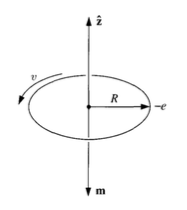
\includegraphics[width=0.94\textwidth]{./images/schematics/orbiting_electron_magnetic_dipole_moment.png}\\
    \end{center}
  \end{column}
  \begin{column}{0.65\textwidth}
     For time intervals much larger than the period of rotation T,
     we may think of the orbiting electron as a {\em steady} current I:
     \begin{equation*}
        I = \frac{q}{T} = - \frac{eu}{2\pi R}
     \end{equation*}
     where u is the electron velocity and R is the radius of its orbit (taken to be circular).
  \end{column}
\end{columns}

\vspace{0.4cm}

The {\bf magnetic dipole moment associated with that orbital motion} is:
\begin{equation*}
  \vec{m} = I \vec{S} = \Big( - \frac{eu}{2\pi R} \Big) \Big( \pi R^2 \hat{z} \Big) \Rightarrow
  \vec{m} = - \frac{1}{2} e u R \hat{z}
\end{equation*}

\end{frame}

%
%
%

\begin{frame}{Physical origin of diamagnetism}

Within an external $\vec{B}$ field, there is a significant effect on the electron orbit.

\begin{columns}
  \begin{column}{0.25\textwidth}
    \begin{center}
      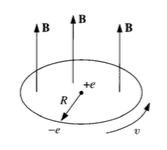
\includegraphics[width=0.90\textwidth]{./images/schematics/orbiting_electron_in_magnetic_field.png}\\
    \end{center}
  \end{column}
  \begin{column}{0.75\textwidth}
     In the absence of a $\vec{B}$ field, Coulomb's force (due to the nucleus) provides centripetal acceleration:
     \begin{equation*}
        \frac{1}{4\pi \epsilon_0} \frac{e^2}{R^2} = m_e \frac{u^2}{R}
     \end{equation*}
  \end{column}
\end{columns}
In the presence of a $\vec{B}$ field, there is an additional force $-e \Big( \vec{u} \times \vec{B} \Big)$.

Assuming (for simplicity) that $\vec{B}$ is perpendicular to the orbital plane, then:
\begin{equation*}
   \frac{1}{4\pi \epsilon_0} \frac{e^2}{R^2} + e \bar{u} B = m_e \frac{\bar{u}^2}{R} \Rightarrow
   m_e \frac{u^2}{R} + e \bar{u} B = m_e \frac{\bar{u}^2}{R} \Rightarrow
\end{equation*}
\begin{equation*}
    e \bar{u} B = \frac{m_e}{R} \Big( \bar{u}^2 - u^2 \Big) \Rightarrow
    e \bar{u} B = \frac{m_e}{R} \Big( \bar{u} + u \Big)  \Big( \bar{u} - u \Big)
\end{equation*}

\end{frame}


%
%
%

\begin{frame}{Physical origin of diamagnetism}

Assuming that the change ${\Delta}u = \bar{u} - u$ is small, so that $\bar{u} + u \approx 2u \approx 2\bar{u}$,
we can write the previous equation as:
\begin{equation*}
    e \bar{u} B = \frac{m_e}{R} \Big( \bar{u} + u \Big)  \Big( \bar{u} - u \Big) \Rightarrow
    e \cancel{\bar{u}} B = \frac{m_e}{R} 2 \cancel{\bar{u}} {\Delta}u \Rightarrow
\end{equation*}
\begin{equation*}
    {\Delta}u = \frac{eRB}{2m_e}
\end{equation*}
In the presence of a $\vec{B}$ field, the electron velocity increases by ${\Delta}u$.
This changes its magnetic dipole moment:
\begin{equation*}
  \vec{m} = - \frac{1}{2} e u R \hat{z}
\end{equation*}
The change $ {\Delta}\vec{m}$ is given by:
\begin{equation*}
    {\Delta}\vec{m} =
      - \frac{1}{2} e {\Delta}u R \hat{z} =
      - \frac{1}{2} e \Big( \frac{eRB}{2m_e} \Big) R \hat{z} \Rightarrow
    {\Delta}\vec{m} =
      - \frac{e^2 R^2}{4m_e} \vec{B}
\end{equation*}

\end{frame}

% ------------------------------------------------------------------------------

%
% Worked example :
%

{
\problemslide

%
%
%

\begin{frame}{Worked example: Free current on circular wire}

  \begin{blockexmplque}{Question}
    An infinite straight wire with a circular cross-section
    of radius $R$ is lying along the $z$ axis
    and it has an internal $\vec{H}$ field given by
    \begin{equation*}
      \vec{H} = \frac{J_0}{r} \Big(\frac{1}{a^2} sin(ar) - \frac{r}{a} cos(ar) \Big) \hat{\phi}
    \end{equation*}
    where
    $r$ is the radial distance from the centre of the circular conductor,
    $\hat{\phi}$ is the azimuthal unit vector,
    $J_0$ is a constant current density,
    and $a$=$\pi/(2R)$.
    Find an expression for the total free current in the conductor,
    and give its direction.
  \end{blockexmplque}

  The free current $I$ can be computed from Ampere's law:
  \begin{equation*}
    I = \oint_{L} \vec{H} \cdot d\vec{\ell}
  \end{equation*}

\end{frame}

%
%
%

\begin{frame}{Worked example: Free current on circular wire}

  Using the given $\vec{H}$ field, and using $a=\pi/2R$, as given,
  the previous expression for $I$ becomes:
  \begin{equation*}
    I = \oint_{L} \frac{J_0}{r}
     \Big(\frac{2R}{\pi^2} sin(\frac{\pi r}{2R}) - \frac{2Rr}{\pi} cos(\frac{\pi r}{2R}) \Big) \hat{\phi}
     \cdot d\vec{\ell}
  \end{equation*}

  To calculate the total free current in the circular conductor, we choose
  a closed circular path with radius equal to the radius of the conductor.
  The element $d\vec{\ell}$ can be written as:
  \begin{equation*}
     d\vec{\ell} = R d\phi \; \hat{\phi}
  \end{equation*}

  Using the above expression for $d\vec{\ell}$, and substituting $r = R$,
  into the our last expression for $I$, we find:
  \begin{equation*}
    I = \int_{0}^{2\pi} \frac{10^4}{R}
     \Big(\frac{4R^2}{\pi^2} sin(\frac{\pi R}{2R}) - \frac{2R^2}{\pi} cos(\frac{\pi R}{2R}) \Big) \hat{\phi}
      \cdot \Big( R d\phi \; \hat{\phi} \Big) \xRightarrow{\hat{\phi} \cdot \hat{\phi} = 1}
  \end{equation*}

\end{frame}

%
%
%

\begin{frame}{Worked example: Free current on circular wire}

  \begin{equation*}
    I = \frac{J_0}{R}
     \Big(\frac{4R^2}{\pi^2} \cancelto{1}{sin(\frac{\pi}{2})} - \frac{2R^2}{\pi} \cancelto{0}{cos(\frac{\pi}{2})} \Big)
      R \int_{0}^{2\pi} d\phi \Rightarrow
  \end{equation*}

  \begin{equation*}
    I = \frac{J_0}{\cancel{R}} \frac{4R^2}{\pi^{\cancel{2}}} \cancel{R} 2\cancel{\pi} \Rightarrow
  \end{equation*}

  \begin{equation*}
    I = \frac{8 J_0}{\pi} R^2
  \end{equation*}

  Since $\vec{H}$ is an azimuthal vector,
  the free current flows in the positive $z$ axis.

\end{frame}

} % Worked example

% ------------------------------------------------------------------------------
% ------------------------------------------------------------------------------

%
% Worked example :
%

{
\problemslide

%
%
%

\begin{frame}{Worked example: Toroid with square iron core}

  \begin{blockexmplque}{Question}
    \begin{minipage}[r]{0.82\textwidth}
      A toroid having an iron core of square cross-section and permeability $\mu$
      is wound with $N$ closely spaced turns of wire carrying a current $I$.
      Find an expression for the magnitude of the magnetisation $M$ everywhere
      inside the iron core.
    \end{minipage}
    \begin{minipage}[l]{0.15\textwidth}
     \begin{center}
       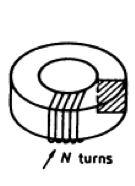
\includegraphics[width=0.94\textwidth]{./images/problems/lect07_toroid_with_square_iron_core}
     \end{center}
    \end{minipage}
  \end{blockexmplque}

  The magnetisation $M$ inside the iron core is:
  \begin{equation*}
    M = \frac{B}{\mu_0} - H
  \end{equation*}

  According to Ampere's circuital law:
  \begin{equation*}
    \oint_{L} \vec{H} \cdot d\vec{\ell} = I_{free} = N I
  \end{equation*}
  where $I_{free}$ is the free current through an open area $S(L)$
  whose boundary is the closed path $L$, and $I$ is the current on
  each of the $N$ windings.

\end{frame}

%
%
%

\begin{frame}{Worked example: Toroid with square iron core}

  Considering the cylindrical symmetry of the problem, $\vec{H}$ is azimuthal.
  Therefore, for a closed path $L$ which is concentric to the iron core,
  perpendicular to the symmetry axis of the toroid,
  and lies within the core:
  \begin{equation*}
    \oint_{L} \vec{H} \cdot d\vec{\ell} = H 2\pi r
  \end{equation*}

  Therefore, Ampere's circuital law yields:
  \begin{equation*}
    H 2\pi r = N I \Rightarrow H = \frac{NI}{2\pi r}
  \end{equation*}

  The magnetic field $B$ can be computed from $H$ as follows:
  \begin{equation*}
     B = \mu H
  \end{equation*}

  Substituting the above into our initial expession for $M$, we find:
  \begin{equation*}
    M = \frac{\mu H}{\mu_0} - H
      = \Big( \frac{\mu}{\mu_0} - 1 \Big) H
      = \Big( \frac{\mu}{\mu_0} - 1 \Big) \frac{NI}{2\pi r}
  \end{equation*}

\end{frame}

} % Worked example


% ------------------------------------------------------------------------------
% ------------------------------------------------------------------------------
